\documentclass[12pt, letterpaper]{article}

\usepackage{color} %% Allows text to be typeset in color.

%% These allow Me to add Images to the Book.
\usepackage{graphicx}
\graphicspath{ {images/} }

%% Enables hyperlinks.
\usepackage{hyperref}

%% Makes BigO easier.
\newcommand{\bigO}{\mathcal{O}}
\newcommand{\bigOmega}{\Omega}
\newcommand{\bigTheta}{\Theta}

%%
\oddsidemargin0cm
\evensidemargin0cm
\topmargin-2cm     % These lines increase the amount of usable space and save trees.
\textwidth16.5cm
\textheight23.5cm  

%%\setcounter{tocdepth}{4} %% set the table of contents detail depth.

%% Types of organizational sections.s
%%\part{}
%%\chapter{}
%%\section{}
%%\subsection{}
%%\subsubsection{}
%%\paragraph{}
%%\subparagraph{}

\begin{document}

\title{\color{blue}Hump Yard Rules v1.4}
\author{Written by Bryce Summers \texttt(BryceSummers.com)}
\date{\color{red}Last Updated: \today}
\maketitle

\tableofcontents 

\section{Overview}

Hump Yard is a game about creating the most efficient rail classification yard possible in order to win more sorting contracts than your opponents.

\newpage
\section{Components}

Hump Yard comes with 4 of each of the following \textit{normal} Track tiles:


\includegraphics[width=0.20\textwidth]{Track_0.png}

\includegraphics[width=0.20\textwidth]{Track_3.png}
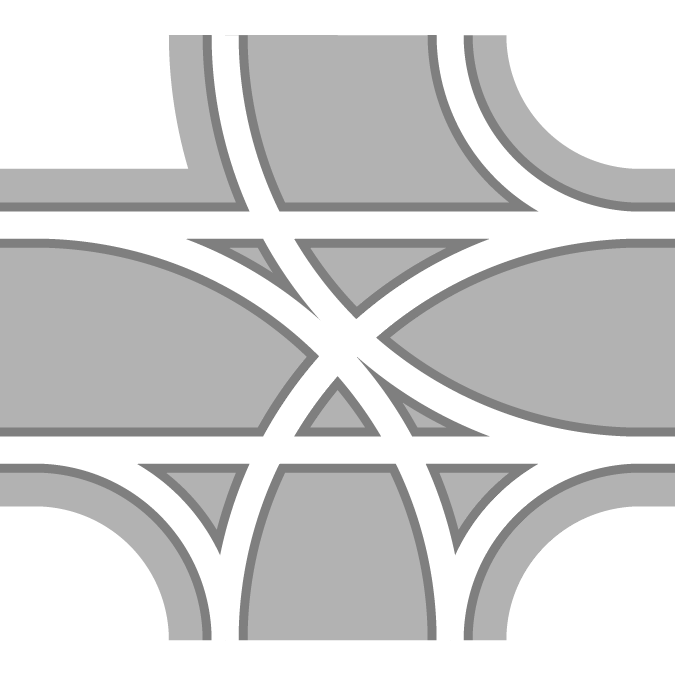
\includegraphics[width=0.20\textwidth]{Track_10.png}
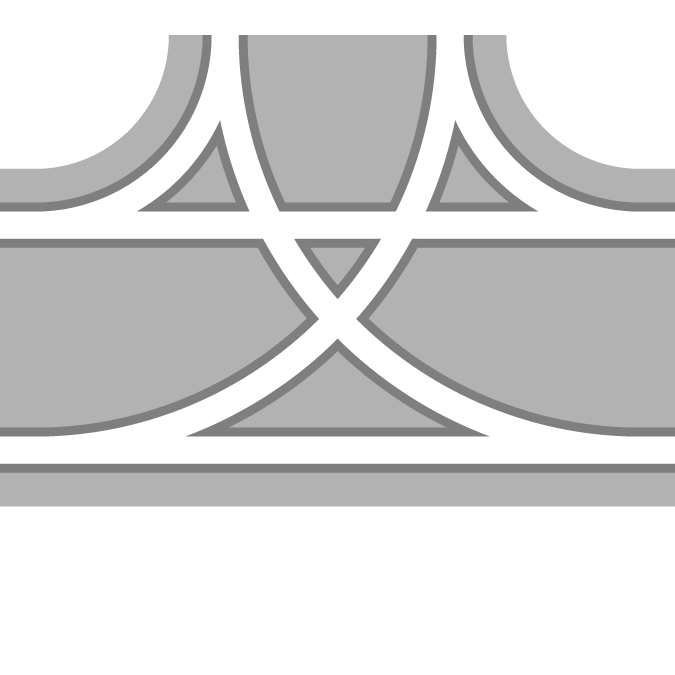
\includegraphics[width=0.20\textwidth]{Track_22.png}

\includegraphics[width=0.20\textwidth]{Track_25.png}
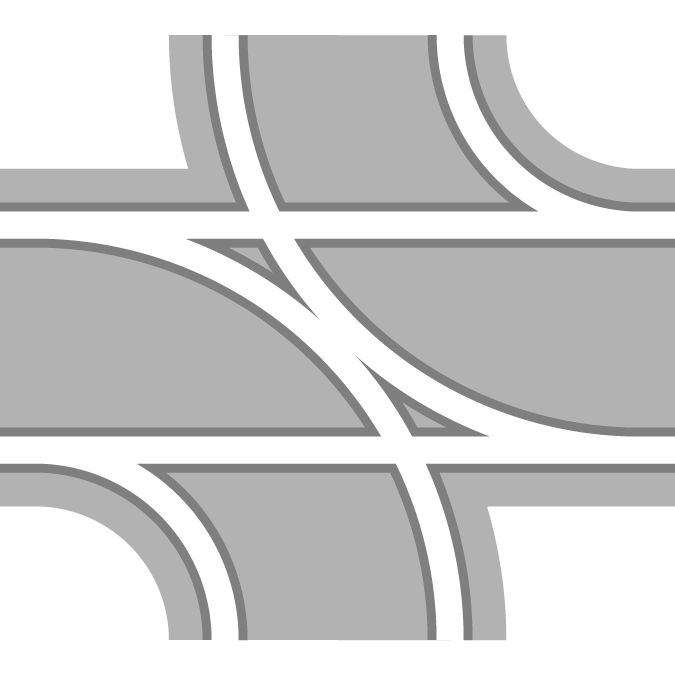
\includegraphics[width=0.20\textwidth]{Track_26.png}

\includegraphics[width=0.20\textwidth]{Track_32.png}

\includegraphics[width=0.20\textwidth]{Track_35.png}
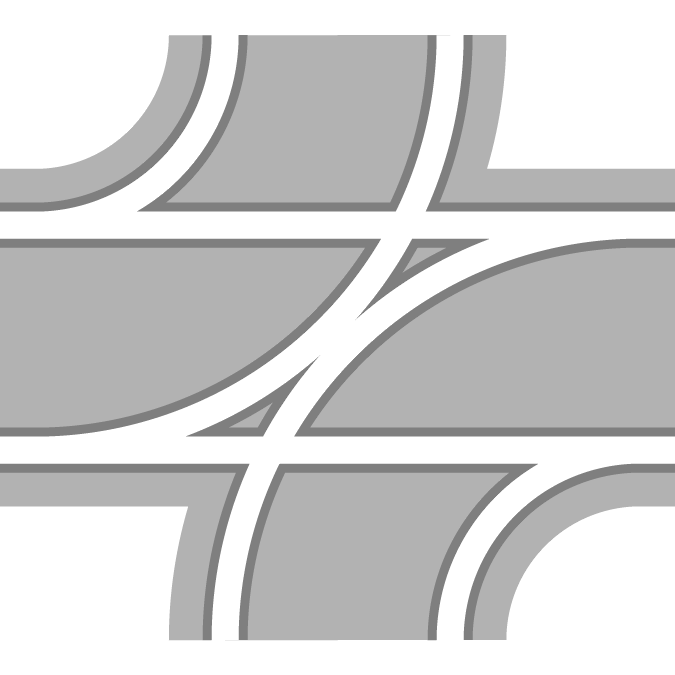
\includegraphics[width=0.20\textwidth]{Track_38.png}

\includegraphics[width=0.20\textwidth]{Track_39.png}

\includegraphics[width=0.20\textwidth]{Track_40.png}

\includegraphics[width=0.20\textwidth]{Track_41.png}

\includegraphics[width=0.20\textwidth]{Track_43.png}
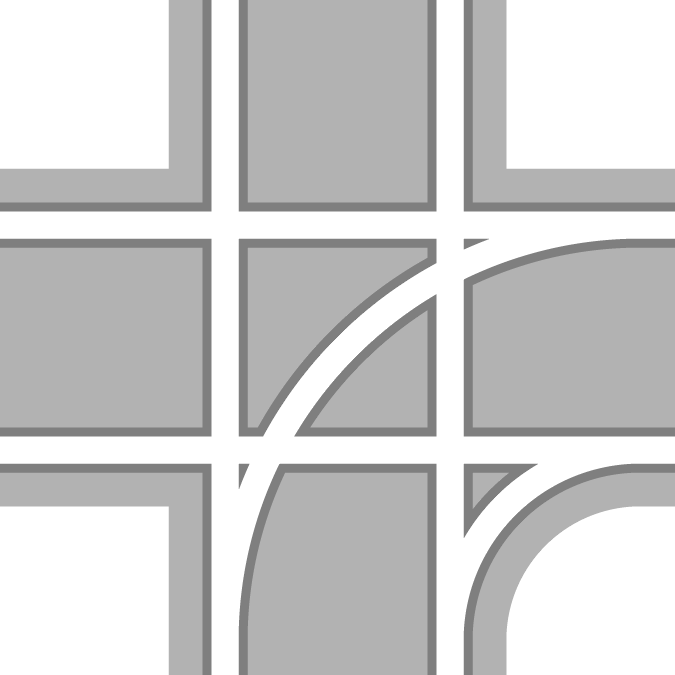
\includegraphics[width=0.20\textwidth]{Track_44.png}

\includegraphics[width=0.20\textwidth]{Track_45.png}

\includegraphics[width=0.20\textwidth]{Track_55.png}

\includegraphics[width=0.20\textwidth]{Track_57.png}
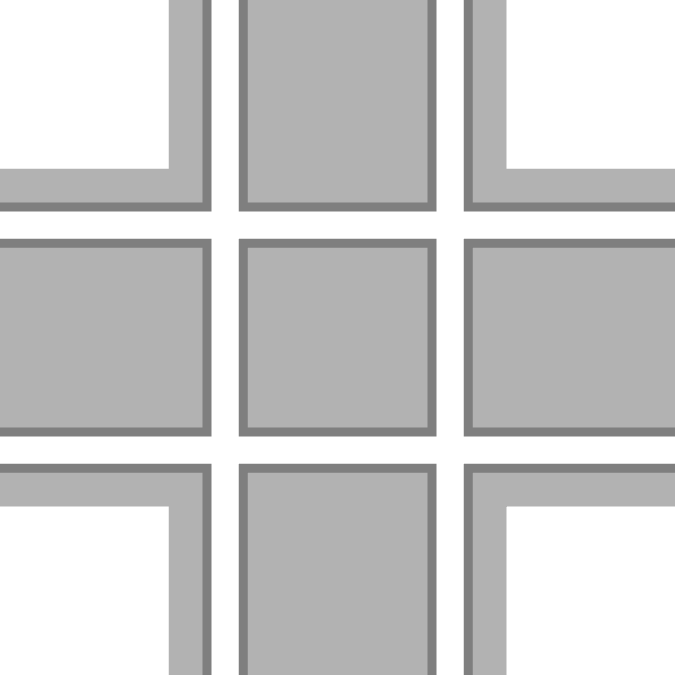
\includegraphics[width=0.20\textwidth]{Track_60.png}
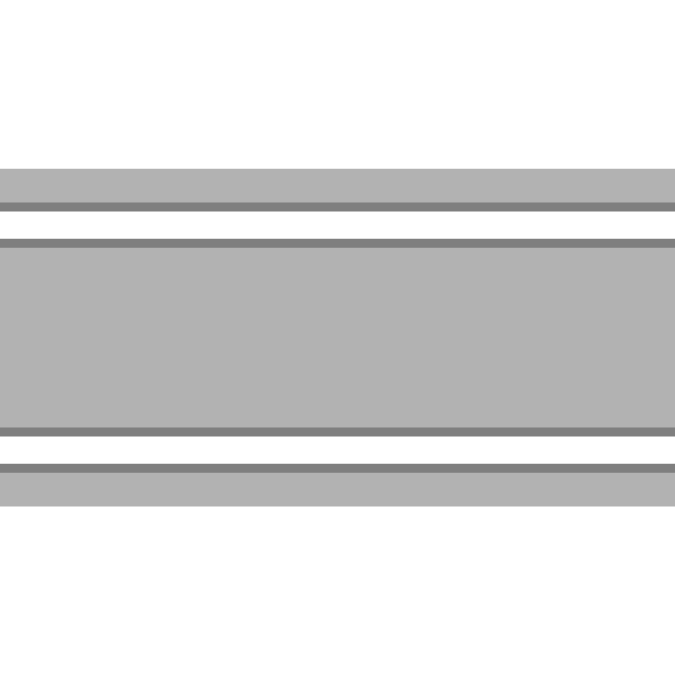
\includegraphics[width=0.20\textwidth]{Track_62.png}
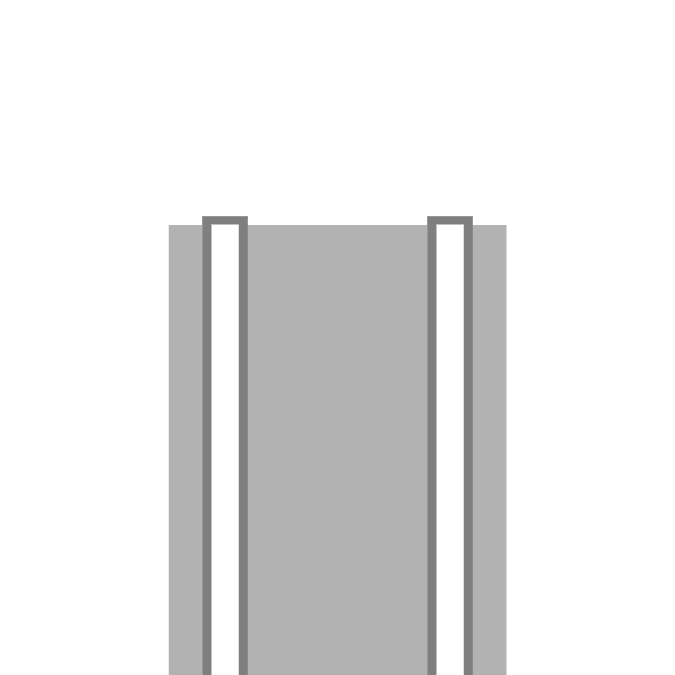
\includegraphics[width=0.20\textwidth]{Track_end.png}

5 of each of the following colored track headings:

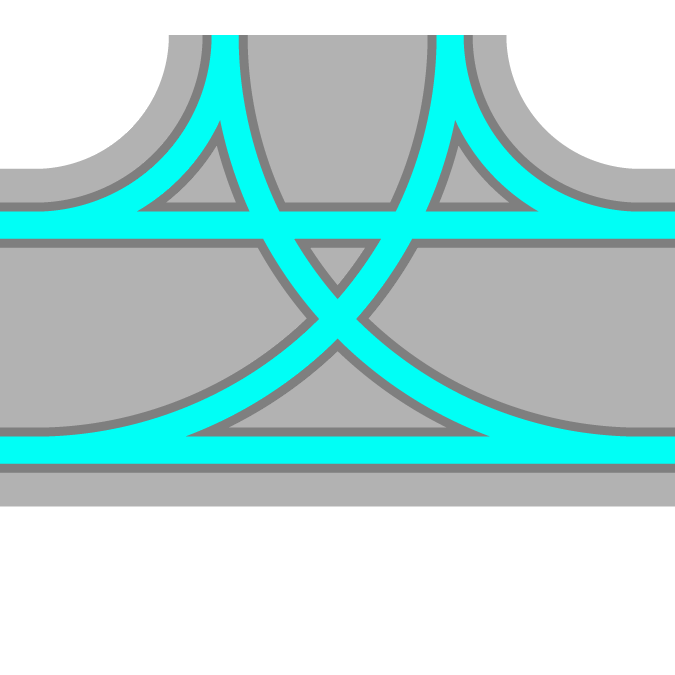
\includegraphics[width=0.20\textwidth]{BlueHeading.png}
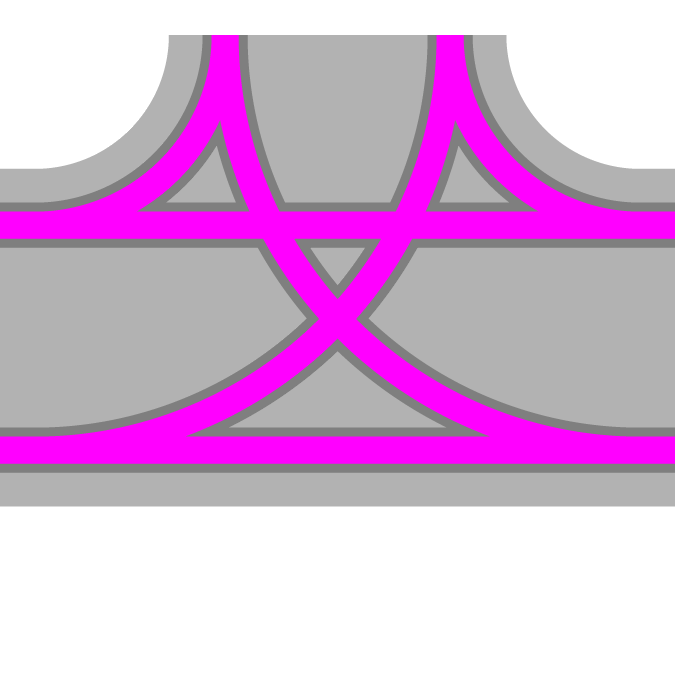
\includegraphics[width=0.20\textwidth]{PurpleHeading.png}
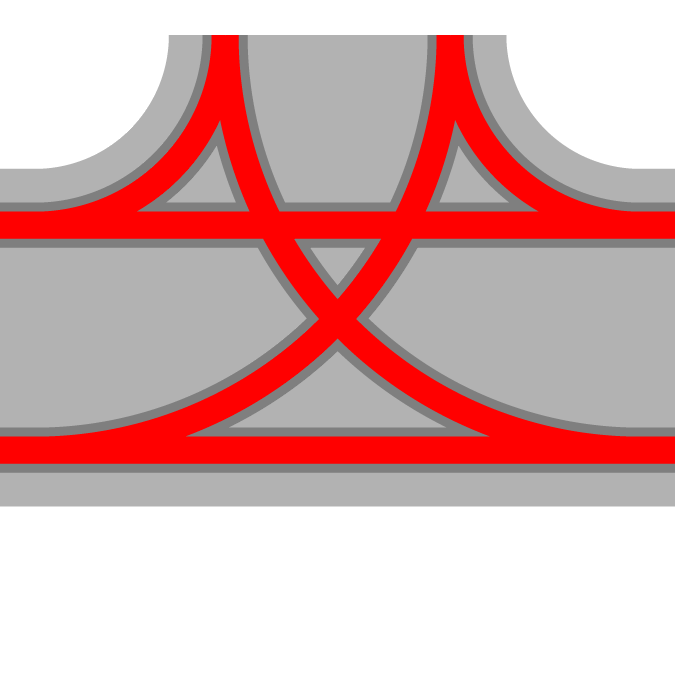
\includegraphics[width=0.20\textwidth]{RedHeading.png}
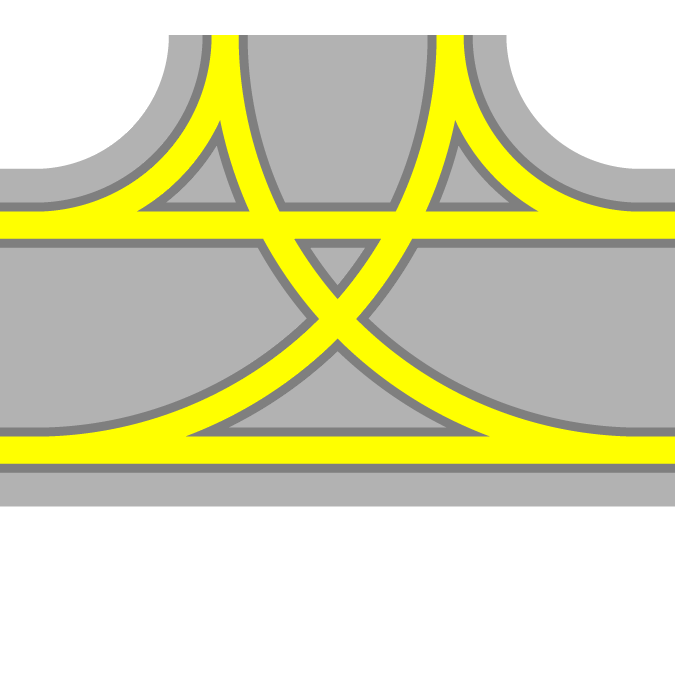
\includegraphics[width=0.20\textwidth]{YellowHeading.png}


%%8 Sources and 8 Sinks.
%%
\includegraphics[width=0.25\textwidth]{Source.png} $\times 8$
%%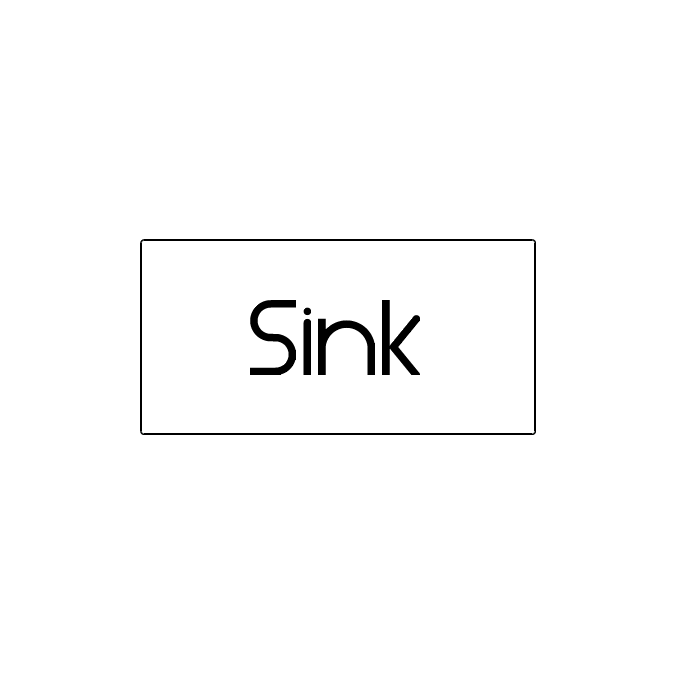
\includegraphics[width=0.25\textwidth]{Sink.png} $\times 8$

Pieces used for the simulation of moves in contract fullfillments, Colorful Car cards used to represent contracts.

\newpage
\section{Rules of Play}

\subsection{Setup}

Every players sets up their yard as follows with 5 of their colored heading tracks :

%%
\includegraphics[width=0.10\textwidth]{Source.png}
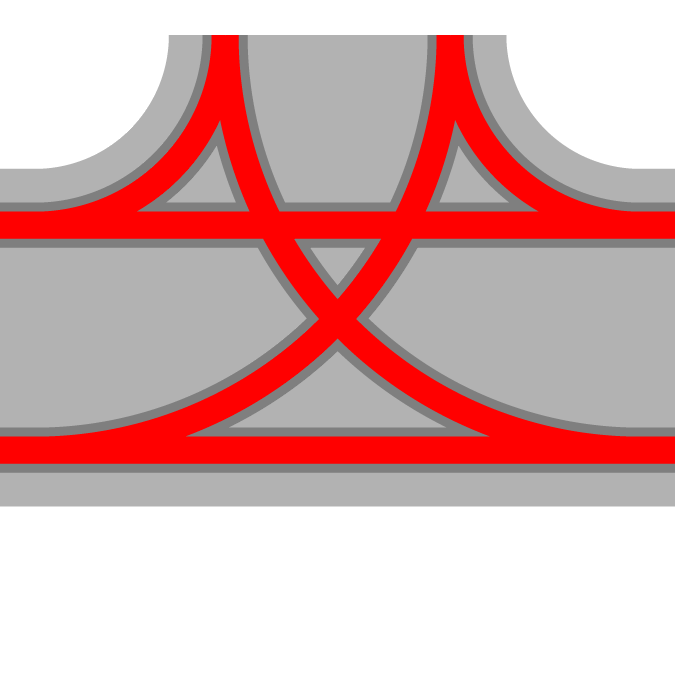
\includegraphics[width=0.10\textwidth]{RedHeading.png}
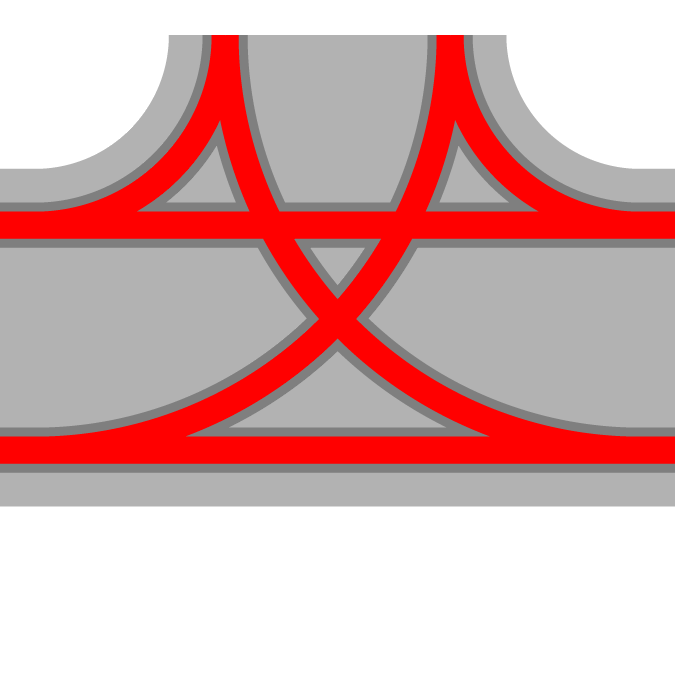
\includegraphics[width=0.10\textwidth]{RedHeading.png}
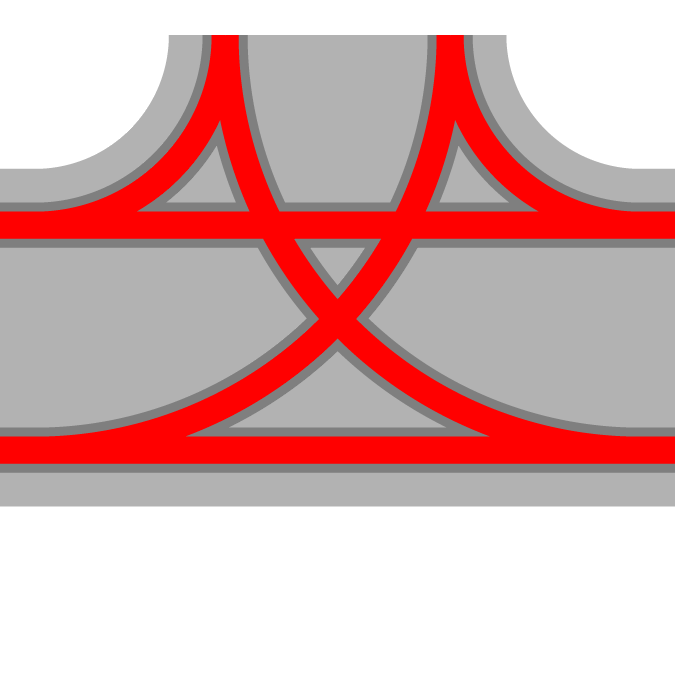
\includegraphics[width=0.10\textwidth]{RedHeading.png}
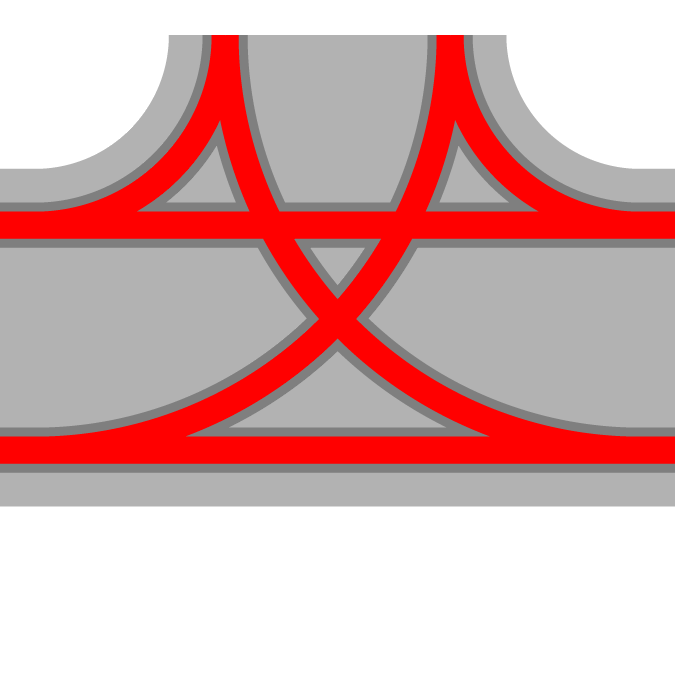
\includegraphics[width=0.10\textwidth]{RedHeading.png}
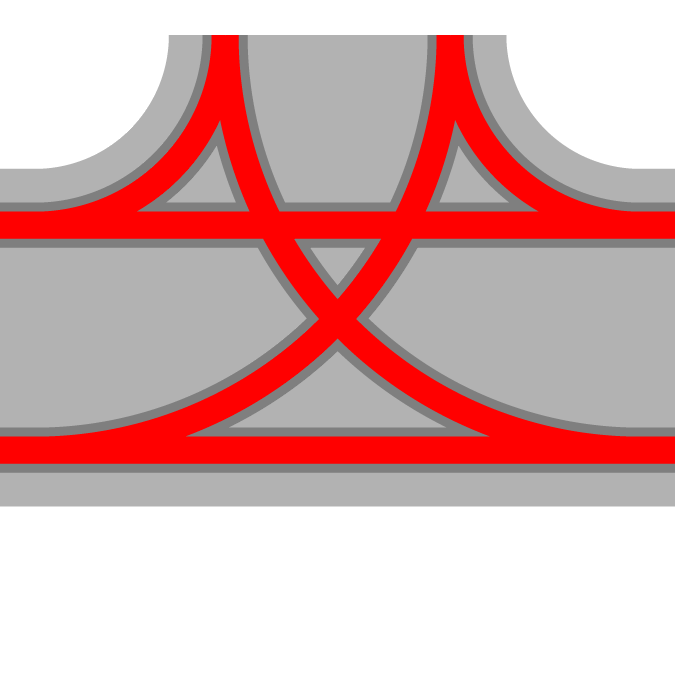
\includegraphics[width=0.10\textwidth]{RedHeading.png}
%%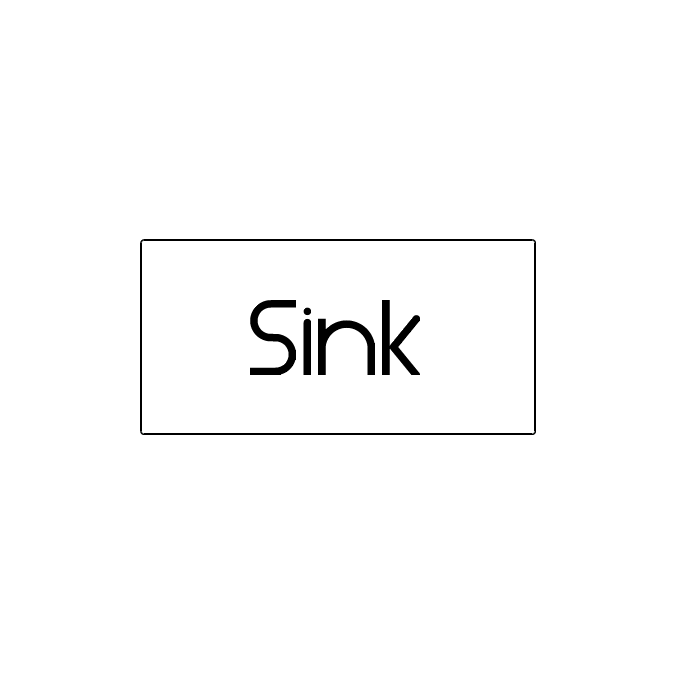
\includegraphics[width=0.10\textwidth]{Sink.png}

It is perfectly fine to have the headings point downwards if desired.

Shuffle all of the track tiles and place them in a stack face down.

Players start the game with 0 points.

Each player is randomly given one free track piece in fo their yard at the start of the game.

Shuffle the deck of car cards and place 3 of them in a line in the center of the table, therebye forming the length 3 contract.

Do the same with the next 4 cards to make the length 4 contract.

\subsection{Turn Order}

At the beginning of the game, the turn order is chosen randomly.\\

At the beginning of every other turn, the turn order is established via the following protocol.

\begin{enumerate}
\item A person with fewer car cards is earlier in turn order.
\item If both people have the same number of car cards, then the person with more tracks is earlier in turn order.
\item If both players had the same number of tracks, then the player who was later in turn order last turn will be earlier in turn order this turn.
\end{enumerate}

\subsection{Turns}

Every turn consists of a sequence of three phases.

\subsubsection{Phase I : Contract Bidding.}

Players bid on the number of moves they think they could use to proccess the train after the order of the cars has been randomly shuffled.

\begin{enumerate}
\item \textbf{Pass} : A player does not compete for any contract.
\item \textbf{Bid} : A player bids the number of moves they think it will take to fullfill a contract.
\item \textbf{Underbid} : A player bids a lower number of moves for a contract previously bid on by another player this turn. They underbidden players are then able to \textbf{pass}, \textbf{bid} on a different contract, \textbf{underbid} any contract (including the one they have been underbidden on), or \textbf{Retain} the overbidden contract.
\item \textbf{Retain} : A player decides to keep their bid on a contract when they have been underbidden and they will be able to attempt to fullfill the contract if all players who have underbidden them fail to fullfill the contract.
\end{enumerate}

\textbf{Note} : No two players may make the same bid for the same contract on the same turn.\\
\textbf{Note} : It is disadvantageous to make a bid that is unlikely to be fullfilled, because players who do this will not be able to perform track construction this turn in Phase III.

All players end phase I with either a bid on a contract or a pass.

\subsubsection{Phase II : Contract Work.}

For every contract with a bet on it this turn, the bidding players will need to attempt to fullfill the contract. The order in which the different contract fullfillments are resovled may be done in any arbitrary order, such as smallest contract to largest contract.

\paragraph{Attempting to fullfill a contract. } A player attempt to fullfill a contract as follows.

\begin{enumerate}
\item Set up a line of colored train pieces in the middle of the table matching the initial order as shown on the cards representing the contract. This is the \textbf{input}  order.
\item Shuffle the contract trains cards and set them back down in the middle of the table. The new order shown is the order of the \textbf{output} train that the client wants the input order sorted into.
\item The player lines up a copy of the input order at one side of their heading tracks.
\item The player must find a sequence of moves that transforms the input into the output such that the number of moves does not exceed the player's bid. The output must be moved as an entire train out of the opposite side of the yard that the input came in on. If the other players are in a friendly mood, they are welcome to help the player think of such as solution. If a player comes up with a proper solution then they \textbf{receive all the contract car cards} and the fullfillment attempt ends and play moves on to the next contract. The player will also receive one \textbf{service token} for every car that stopped at a service track of the appropiate color. A new contract must be generated by placing $n + 1$ cards in the middle of the table, where $n$ is the length of the previous largest of the two contracts on the table. In this manner, the contracts in the game will be availible in the order of length 3, 4, 5, 6, 7, 8, 9, and 10.
\item If the player cannot think of a solution, then they have failed to fullfill the contract. In the event of a failed contract, the retaining players in order of increasing bid will have a chance to fulfill the contract.  The retaining players should skip steps 1 and 2 so that they have the same input order and output order requirements as the lowest bidder had.
\end{enumerate}

Once all fullfillment attempts have been resolved, play proceeds to Phase III.

\subsubsection{Phase III : Track Construction}

Players perform phase III in turn order depending on the following cases:

\begin{enumerate}
\item If a player passed in Phase I this turn, then they may buy and build 2 pieces of track.
\item If a player failed to fullfill a contract this turn, then they may not build any pieces of track this turn.
\item Any players who fullfilled their contracts this turn, or who retained a contract that was fullfilled by another player, may buy and build 1 piece of track this turn.
\end{enumerate}

\paragraph{Buying and Building a track piece. }

The track market is created each turn by randomly placing 2 face up pieces of track per player in the game in the middle of the table. In turn order, players may buy a track piece simply by choosing one of these tiles. They may then build it by rotating it however they desire and placing it next to any piece of track currently in their yard vertically or horizontally.

\paragraph{Note: } Every piece of track that you add to your yard will likely minimize the amount of moves it will take to fullfill future contracts.

\subsection{End of Game}

The game ends at the end of a turn if one of the following two conditions are met:

\begin{enumerate}
\item A player has 20 tracks in their yard, not counting the initial heading tracks.
\item All contracts have been fullfilled.
\end{enumerate}

\subsection{Winner}

At the end of the game, the winner is the player with the most points. A player gets 1 point for every car they have aquired and 1 point for every service token they have aquired.

\section{Legal Moves}

A set of connected cars may be moved as far as possible in one direction. Cars may be interpreted as coupled or uncoupled at the beginning of the move, but the interpretation cannot be changed until the next moves, in other words if you wish to move and connect cars, you will have to move the first train to the other train, then end the move. During your next move, you may interpret the cars as coupled into one train.

To properly exit a train from the yard, every car must be coupled and be in the order specified by the random permuation.

A train may go around loops. Cars may be "humped" into the yard in groups of any size.
A person may hump them each individually, or hump multiple cars at the same time.
Trains may not intersect themselves during a move.
Cars may not inhabit the same tile as any other car during a move unless the two cars are on opposite curves.

\section{Servicing Tracks}

Straight pieces of track should grant bonuses for a color of car that stops on them.

\section{Terminology}

\begin{enumerate}
\item Heading track.
\item Fullfilling a contract.
\item Input order
\item Output order
\item Servicing a car
\item Yard.
\item Track Market.
\item Retaining player.
\item Servicing Tracks.
\item interpret
\item Retaining Player
\item Permutation
\item Humped
\end{enumerate}

Start and end tiles should be used to help clarify the orientation of the trains and yards.

%% Signals that the document has ended.
\end{document}